\section{Introduction to Power Semiconductor Devices}
\title[Introduction to power semiconductor devices]{Introduction to power semiconductor devices}  

\begin{frame}[plain]
    \titlepage
\end{frame}

\begin{frame}{\textbf{Normal vs Power Semiconductor Devices: Key Differences}}
    \textbf{1. Physical Design:}
    \begin{itemize}
        \item \textbf{Normal Devices:} Small device areas, thin active regions for fast operation.
        \item \textbf{Power Devices:} Large device areas, thick drift regions to support high voltages; trade-off between speed and ruggedness.
    \end{itemize}

    \textbf{2. Key Parameters:}
    \begin{itemize}
        \item \textbf{Normal Devices:} Optimize \textit{speed}, \textit{gain}, \textit{integration density}.
        \item \textbf{Power Devices:} Optimize \textit{breakdown voltage}, \textit{on-resistance}, \textit{thermal management}.
    \end{itemize}

    \textbf{3. Material and Fabrication:}
    \begin{itemize}
        \item \textbf{Normal Devices:} Primarily Silicon (Si).
        \item \textbf{Power Devices:} Silicon (Si), but also wide bandgap materials like Silicon Carbide (SiC) and Gallium Nitride (GaN) for superior performance.
    \end{itemize}

    \textbf{4. Examples:}
    \begin{itemize}
        \item \textbf{Normal Devices:} CMOS transistors, Bipolar Junction Transistors (BJTs).
        \item \textbf{Power Devices:} MOSFETs, IGBTs, Diodes (Schottky, PIN), SiC MOSFETs, GaN HEMTs.
    \end{itemize}

    \vspace{0.3cm}
    \textbf{Summary:} \\
    \textit{While normal semiconductors are optimized for information processing, power semiconductors are engineered for robust control of large electrical energy flows.}
\end{frame}


%%%%%%%%%%%%%%%%%%%%%%%%%%%%%%%%%%%%%%%%%%%%%%%%%%%%%%%%%%%%%
%% Conceptual idea of power semiconductor devices physics %%
%%%%%%%%%%%%%%%%%%%%%%%%%%%%%%%%%%%%%%%%%%%%%%%%%%%%%%%%%%%%%
\begin{frame}
	\frametitle{Conceptual idea of a power semiconductor devices physics}
    \textbf{1. Charge Carriers:} 
    \begin{itemize}
        \item Power devices rely on the transport of \textbf{electrons} and \textbf{holes}.
        \item Key mechanisms: \textbf{drift} (due to electric fields) and \textbf{diffusion} (due to concentration gradients).
    \end{itemize}

    \textbf{2. Energy Bands and Junctions:}
    \begin{itemize}
        \item Junctions (e.g., p-n junctions, Schottky barriers) control carrier flow.
        \item Band bending creates potential barriers essential for device blocking and switching behavior.
    \end{itemize}

    \textbf{3. Electric Field Distribution:}
    \begin{itemize}
        \item High electric fields are engineered to manage breakdown and switching.
        \item \textbf{Critical electric field} (\( E_{crit} \)) defines breakdown limits.
    \end{itemize}
\end{frame}


\begin{frame}
	\frametitle{Conceptual idea of a power semiconductor devices physics cond.. }
\textbf{4. Key Physical Processes:}
\begin{itemize}
    \item \textbf{Avalanche Multiplication:} Carrier generation at high fields.
    \item \textbf{Recombination-Generation:} Determines carrier lifetimes.
    \item \textbf{Tunneling:} Important in very high field conditions (Zener breakdown).
\end{itemize}

\textbf{5. Device Performance Metrics:}
\begin{itemize}
    \item \textbf{Blocking Voltage:} Ability to withstand high reverse voltages.
    \item \textbf{On-State Resistance:} Determines conduction losses.
    \item \textbf{Switching Speed:} Influenced by carrier lifetimes and device capacitances.
\end{itemize}

\textbf{Summary:} \\
\textit{Power semiconductor devices are engineered by carefully controlling material properties, doping profiles, junction designs, and carrier dynamics to optimize switching behavior, conduction losses, and voltage handling capabilities.}
\end{frame}

\begin{frame}
	\frametitle{Classification of types of power semiconductor devices}
    \textbf{Based on number of terminals:}
    \begin{columns}
        \column{0.35\textwidth}
        \begin{itemize}
            \item \textbf{Two-terminal devices:}
            \begin{itemize}
                \item Diodes (e.g., Schottky, Zener, and standard rectifier diodes).
            \end{itemize}
            \item \textbf{Three-terminal devices:}
            \begin{itemize}
                \item Insulated Gate Bipolar Transistor (IGBT).
                \item Thyristors (SCRs).
            \end{itemize}
            \item \textbf{Four-terminal devices:}
            \begin{itemize}
                \item IGBT with Kelvin connection.
                \item Cascode structures (e.g., GaN HEMT with a low-voltage MOSFET).
            \end{itemize}
        \end{itemize}

        \column{0.65\textwidth}
        \begin{figure}
            \centering
            \label{fig:Classification_based_on_number_of_terminals}
            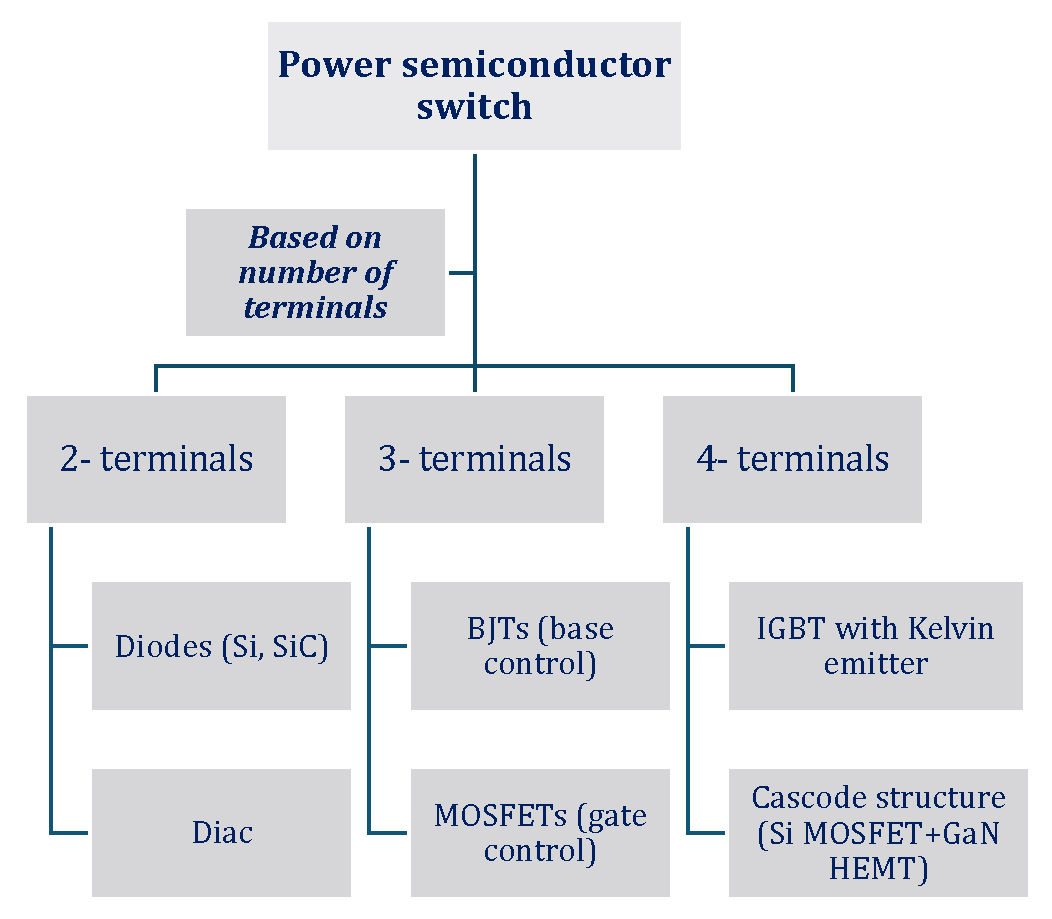
\includegraphics[scale=0.35]{fig/lec04/classification_of_device_1.eps}
            \caption{Classification of power semiconductor devices based on number of terminals.}
        \end{figure}
    \end{columns}
\end{frame}


\begin{frame}
	\frametitle{Classification of types of power semiconductor devices}
    \textbf{Based on number of layser/junctions:}
    \begin{columns}
        \column{0.35\textwidth}
        \begin{itemize}
            \item \textbf{Two-layer devices:}
            \begin{itemize}
                \item Diodes (e.g., Schottky, Zener, and standard rectifier diodes).
            \end{itemize}
            \item \textbf{Three-layers devices:}
            \begin{itemize}
                \item BJTs.
                \item MOSFETs.
            \end{itemize}
            \item \textbf{Four-layers devices:}
            \begin{itemize}
                \item GTOs
                \item SCRs.
            \end{itemize}
        \end{itemize}

        \column{0.65\textwidth}
        \begin{figure}
            \centering
            \label{fig:Classification_based_on_number_of_layers}
            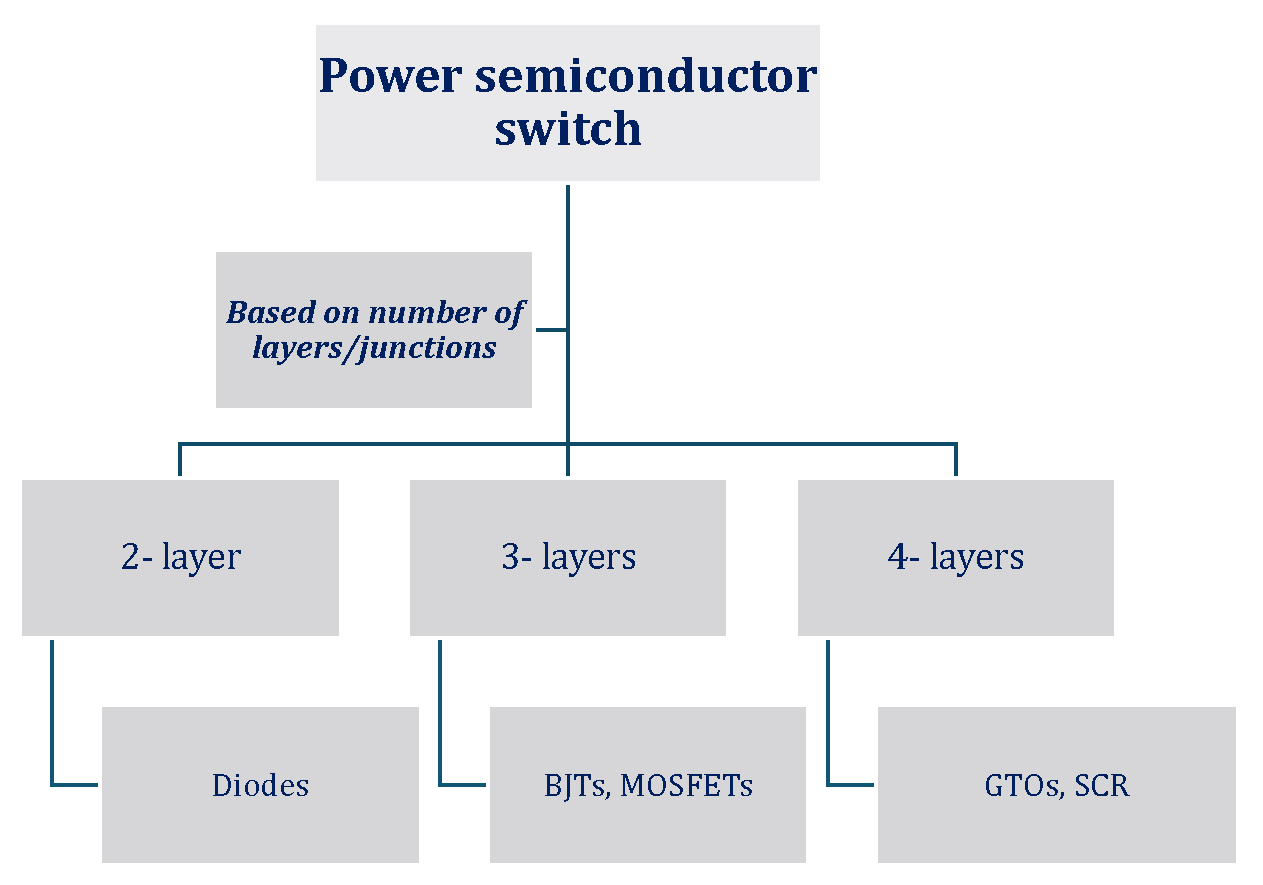
\includegraphics[scale=0.35]{fig/lec04/classification_of_device_2.eps}
            \caption{Classification of power semiconductor devices based on number of layers.}
        \end{figure}
    \end{columns}
\end{frame}

\begin{frame}
	\frametitle{Classification of types of power semiconductor devices}
    \textbf{Based on controllability:}
    \begin{columns}
        \column{0.35\textwidth}
        \begin{itemize}
            \item \textbf{Uncontrolled:}
            \begin{itemize}
                \item Diodes (e.g., Schottky, Zener, and standard rectifier diodes).
            \end{itemize}
            \item \textbf{Semicontrolled:}
            \begin{itemize}
                \item SCRs.
            \end{itemize}
            \item \textbf{Fully controlled:}
            \begin{itemize}
                \item BJTs.
                \item MOSFETs.
            \end{itemize}
        \end{itemize}

        \column{0.65\textwidth}
        \begin{figure}
            \centering
            \label{fig:Classification_based_on_controllability}
            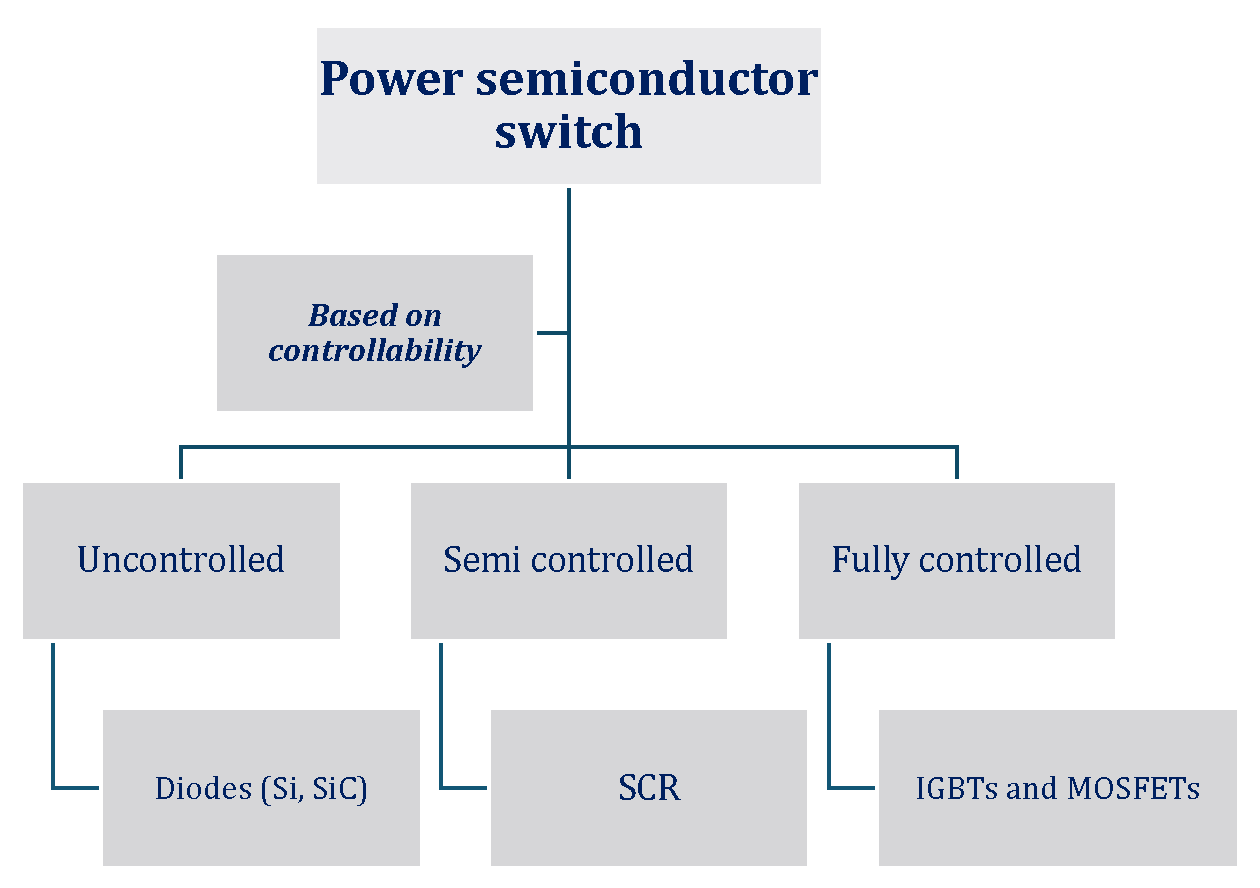
\includegraphics[scale=0.35]{fig/lec04/classification_of_device_3.eps}
            \caption{Classification of power semiconductor devices based on controllability.}
        \end{figure}
    \end{columns}
\end{frame}


\begin{frame}
	\frametitle{Classification of types of power semiconductor devices}
    \textbf{Based on quadrant of operation:}
    \begin{columns}
        \column{0.35\textwidth}
        \begin{itemize}
            \item \textbf{Single quadrant:}
            \begin{itemize}
                \item Diodes (e.g., Schottky, Zener, and standard rectifier diodes).
            \end{itemize}
            \item \textbf{Two quadrant:}
            \begin{itemize}
                \item Current bidirectional devices (e.g., MOSFETs).
                \item Voltage bidirectional devices (e.g., MOSFET with a series diodes).
            \end{itemize}
            \item \textbf{Four quadrant:}
            \begin{itemize}
                \item By combination of two or more devices (e.g., using IGBTs and MOSFETs).
                \item MOSFETs.
            \end{itemize}
        \end{itemize}

        \column{0.65\textwidth}
        \begin{figure}
            \centering
            \label{fig:Classification_based_on_quadrant_of_operation}
            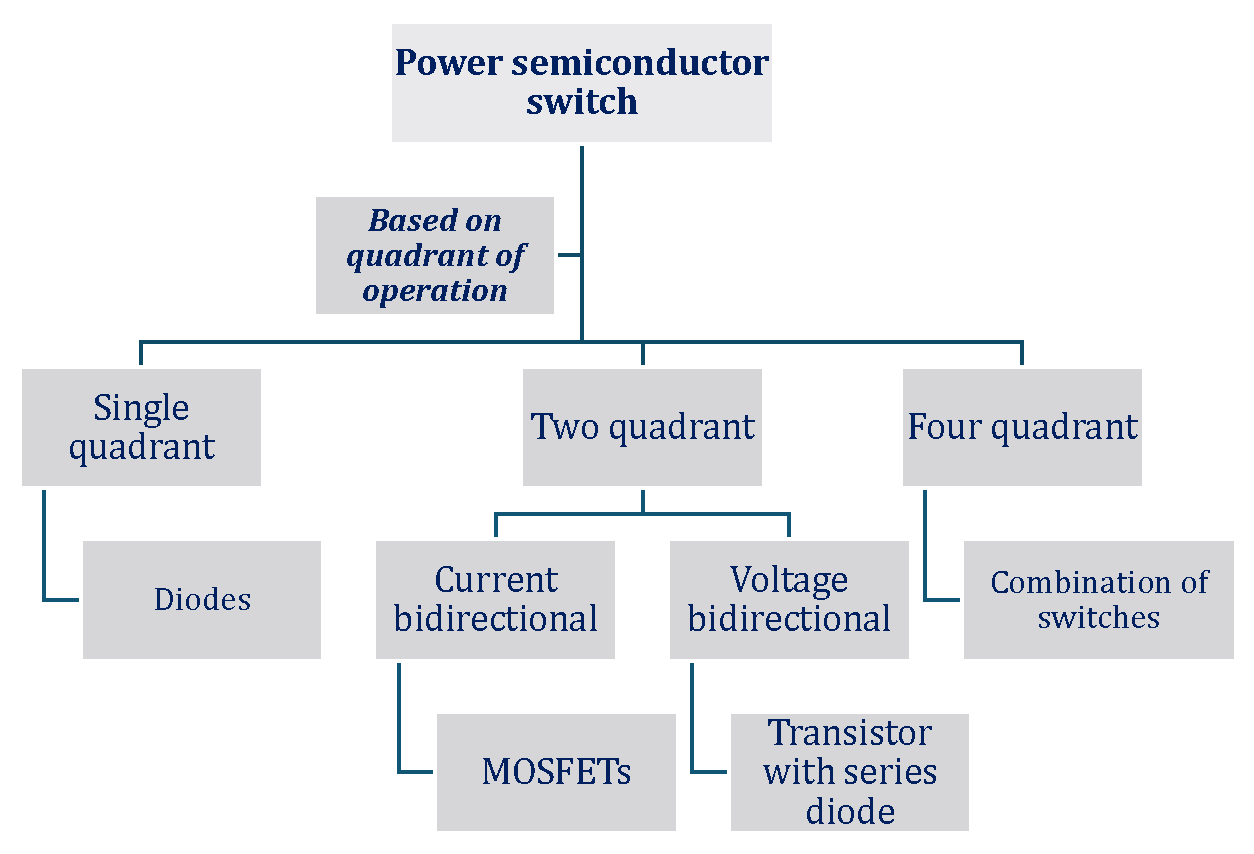
\includegraphics[scale=0.35]{fig/lec04/classification_of_device_4.eps}
            \caption{Classification of power semiconductor devices based on quadrant of operation.}
        \end{figure}
    \end{columns}
\end{frame}

%%%%%%%%%%%%%%%%%%%%%%%%%%%%%%%%%%%%%%%%%%%%%%%%%%%%%%%%%%%%%%%
%% Power Diodes %%
%%%%%%%%%%%%%%%%%%%%%%%%%%%%%%%%%%%%%%%%%%%%%%%%%%%%%%%%%%%%%%%
\begin{frame}
    \frametitle{Power Diodes}
    \textbf{1. Definition:} \\
    \textit{A power diode is a semiconductor device that allows current to flow in one direction while blocking it in the opposite direction. It is designed to handle high voltages and currents, making it suitable for power applications.}

    \textbf{2. Key Characteristics:}
    \begin{itemize}
        \item \textbf{Forward Voltage Drop (\(V_f\)):} The voltage drop across the diode when it is conducting.
        \item \textbf{Reverse Breakdown Voltage (\(V_{BR}\)):} The maximum reverse voltage the diode can withstand before breakdown occurs.
        \item \textbf{Reverse Recovery Time (\(t_{rr}\)):} The time taken for the diode to switch from conducting to blocking state.
    \end{itemize}

    \textbf{3. Types of Power Diodes:}
    \begin{itemize}
        \item \textbf{Standard Rectifier Diodes:} Used in AC-DC conversion.
        \item \textbf{Schottky Diodes:} Low forward voltage drop and fast switching; used in high-frequency applications.
        \item \textbf{Zener Diodes:} Used for voltage regulation and protection against overvoltage conditions.
    \end{itemize}
\end{frame}

\begin{frame}
    \frametitle{Power Diodes- basic structure}
    \begin{columns}
        \column{0.4\textwidth}
        \begin{itemize}
            \item \textbf{Basic Structure:}
            \begin{itemize}
                \item Inclusion of a lightly doped $n^-$ drift region.
                \begin{itemize}
                    \item the lightly doped $n^-$ layer (drift region) allows the depletion region to expand widely under reverse bias.
                    \item Allows the diode to have high voltage blocking capability
                \end{itemize}
                \item Thick epitaxial layer and high current capacity.
                \begin{itemize}
                    \item Epitaxial growth and cross-sectional area are tailored to high current rating.
                    \item Larger devices use 4-inch wafers.
                \end{itemize}
            \end{itemize}
        \end{itemize}

        \column{0.6\textwidth}
        \begin{figure}
            \centering
            \label{fig:Power_Diodes_structure_and_IV_characteristics}
            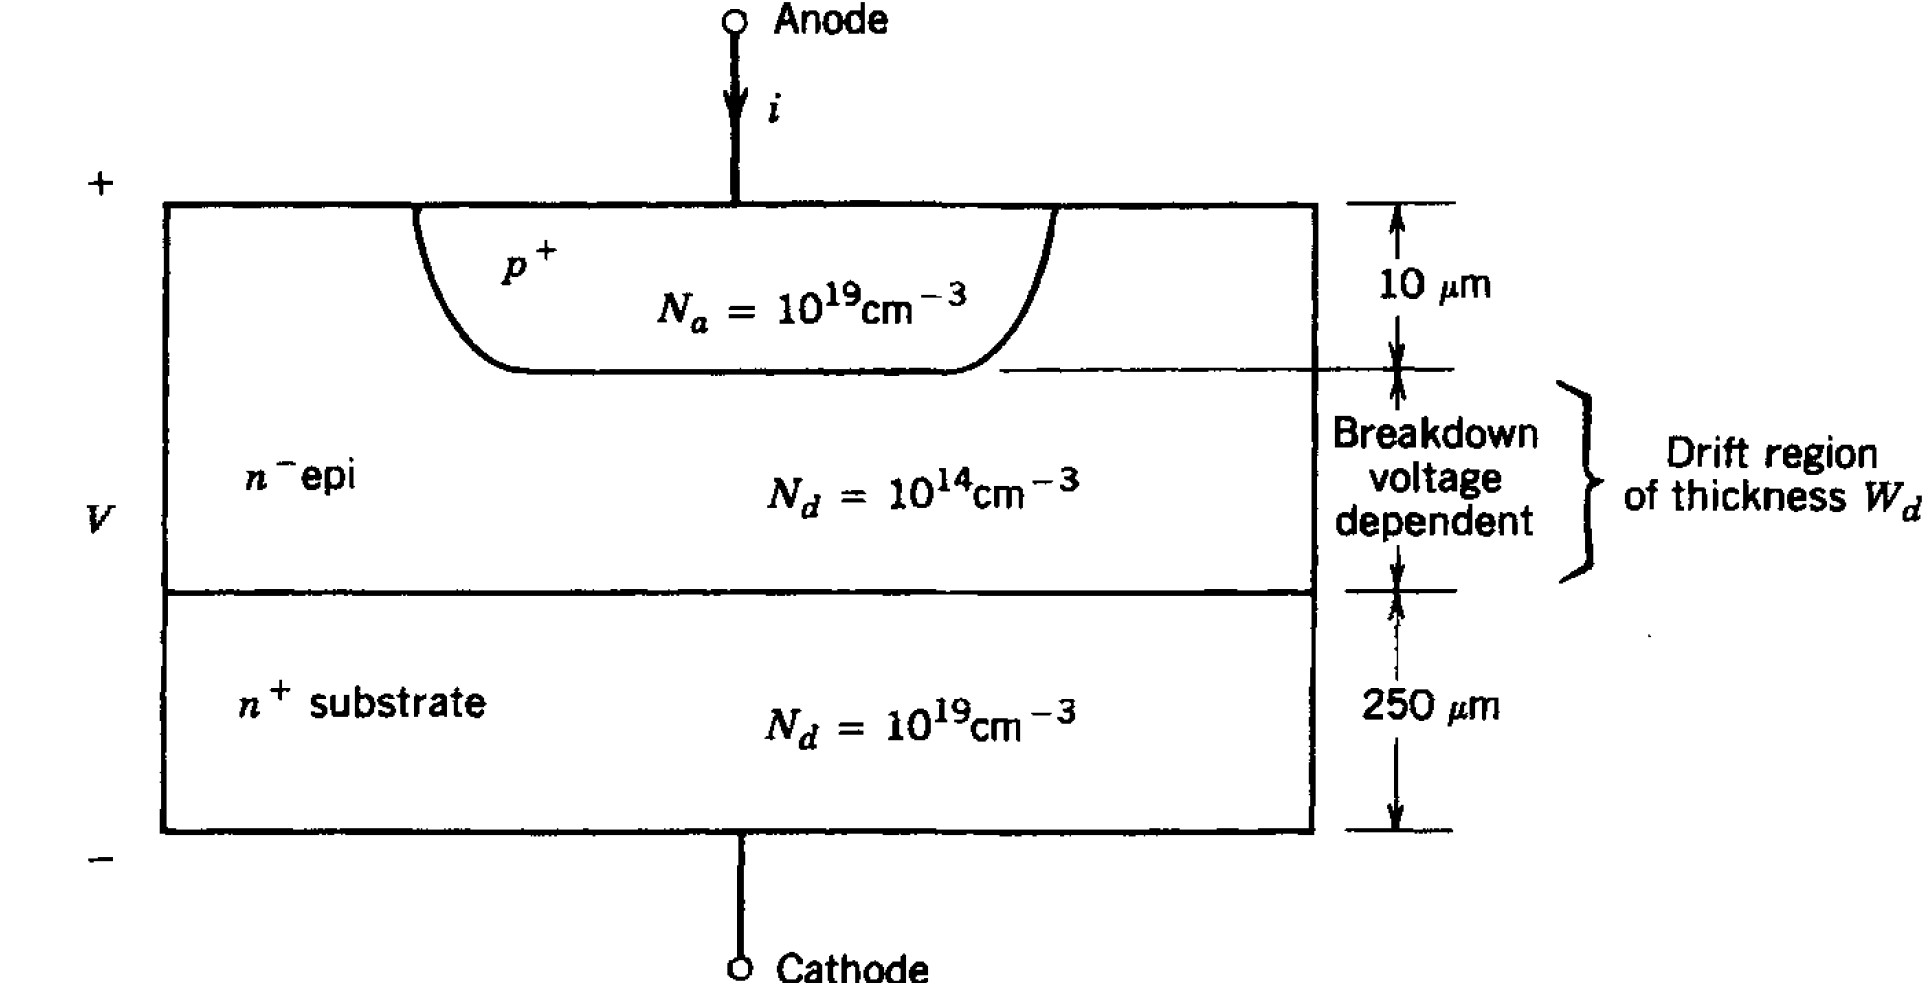
\includegraphics[scale=0.2]{fig/lec04/cross_section_pn_junction.png}
            \caption{Cross section of pn junction diode; adapted from Mohan, Undeland, Robbins, "Power Electronics: Converters, Applications and Design - 2nd Edition".}
        \end{figure}
    \end{columns}
\end{frame}

\begin{frame}{\textbf{Introduction to punch-through vs non-punch-through power diodes}}
    \textbf{Differences:Punch through vs non-punch-through:} 
    \centering
    \small
    \begin{tabular}{|p{3.5cm}|p{4cm}|p{4cm}|}
    \hline
    \textbf{Characteristic} & \textbf{Punch-through (PT)} & \textbf{Non-punch-through (NPT)} \\
    \hline
    Drift Region & Thinner, moderately doped & Thicker, lightly doped \\
    \hline
    Electric Field Profile & Extends through drift region (reaches anode) & Ends before reaching the anode \\
    \hline
    Breakdown Mechanism & Abrupt avalanche breakdown & Gradual breakdown onset \\
    \hline
    Switching Speed & Faster reverse recovery & Slower but more robust \\
    \hline
    On-State Voltage Drop & Lower & Slightly higher \\
    \hline
    Reverse Recovery Loss & Lower & Higher \\
    \hline
    Application Voltage Range & Medium (e.g., 600–1200 V) & High (e.g., >1200 V) \\
    \hline
    Example Devices & Transient Voltage Suppression and Schottky barrier diodes & 1N400x  \\
    \hline
    \end{tabular} \\
    \vspace{0.3cm}
    \textbf{Design Implication:} Choice depends on switching frequency, voltage class, and thermal constraints.
\end{frame}

\begin{frame}{\textbf{Avalanche Breakdown in Step Junctions}}
    \textbf{Concept:} Reverse bias in a $p$–$n$ junction causes the electric field to drop entirely across the depletion region. As the field strength increases, it approaches a critical value $E_{\text{BD}}$ where impact ionization begins $\Rightarrow$ Avalanche Breakdown.
    
    \vspace{0.3em}
    \textbf{Key Definitions:}
    \begin{itemize}
        \item \textbf{Breakdown Voltage} ($BV_{\text{BD}}$): Reverse-bias voltage at which impact ionization becomes significant.
        \item \textbf{Critical Field Strength} ($E_{\text{BD}}$): Electric field at which avalanche multiplication starts.
    \end{itemize}
    
    \vspace{0.3em}
    \textbf{Breakdown Condition:}
    \begin{equation}
        E_{\max} \approx E_{\text{BD}}
    \end{equation}
    \textbf{Where:}
    \begin{itemize}
        \item $E_{\max}$: Maximum electric field in the depletion region.
    \end{itemize}
\end{frame}
    
\begin{frame}{\textbf{Breakdown Voltage Expression for Step Junction}}
    \begin{equation}
    BV_{\text{BD}} = \phi_c + \left[ \frac{W_0 E_{\text{BD}}}{2 \varepsilon} \right]^2 - \phi_c \approx \frac{\varepsilon (N_A + N_D) E_{\text{BD}}^2}{2 q N_A N_D}
    \end{equation}
    
    \textbf{Parameters:}
    \begin{itemize}
        \item $W_0$: Depletion width
        \item $E_{\text{BD}}$: Breakdown electric field
        \item $\varepsilon$: Permittivity of the semiconductor
        \item $N_A, N_D$: Acceptor and donor concentrations
        \item $q$: Electron charge
        \item $\phi_c$: Contact potential
    \end{itemize}
    
    \vspace{0.3em}
    \textbf{Observation:} Breakdown voltage depends strongly on doping concentrations and junction profile (e.g., step, graded, diffused).
\end{frame}


\begin{frame}{\textbf{Breakdown Voltage in Non-Punch-Through (NPT) Diodes}}

    \textbf{Structure Concept:}
    \begin{itemize}
        \item \textbf{Non-punch-through diode:} Drift region thickness $W_d$ is \textit{greater than} depletion width at breakdown.
        \item Depletion region does \textbf{not reach} the heavily doped $n^+$ substrate.
    \end{itemize}
    
    \vspace{0.4em}
    \textbf{Simplified Breakdown Voltage Equation:}
    \begin{equation}
        BV_{\text{BD}} \approx \frac{\varepsilon E_{\text{BD}}^2}{2 q N_D}
    \end{equation}
    \begin{itemize}
        \item $E_{\text{BD}}$: Breakdown electric field
        \item $N_D$: Doping concentration of drift region (lightly doped $n$)
        \item $\varepsilon$: Permittivity of the semiconductor
    \end{itemize}
    
\end{frame}

\begin{frame}{\textbf{Breakdown Voltage in Non-Punch-Through (NPT) Diodes}}

\textbf{Numerical Estimation for Silicon:}
\begin{equation}
    BV_{\text{BD}} \approx \frac{1.3 \times 10^{17}}{N_D}
\end{equation}
(for $N_D$ in $\text{cm}^{-3}$, $BV_{\text{BD}}$ in volts)

\vspace{0.4em}
\textbf{Depletion Width at Breakdown:}
\begin{equation}
    W_d \approx \frac{2 BV_{\text{BD}}}{E_{\text{BD}}} \approx 10^{-5} BV_{\text{BD}} \quad \text{(in cm)}
\end{equation}

\vspace{0.4em}
\textbf{Design Implications:}
\begin{itemize}
    \item High breakdown voltages $\Rightarrow$ require very \textbf{light doping} ($\sim 10^{14}$ cm$^{-3}$).
    \item Drift region width for 1000 V breakdown $\approx$ 100 $\mu$m.
    \item Trade-off between \textbf{blocking capability} and \textbf{on-resistance}.
\end{itemize}
\end{frame}

\begin{frame}{\textbf{Punch-Through Diode Breakdown Mechanism}}
    \begin{columns}
    
    \begin{column}{0.5\textwidth}
    \textbf{Definition:} Punch-through occurs when the reverse bias extends the depletion region entirely across the lightly doped $n^-$ drift region up to the heavily doped $n^+$ region.
    
    \begin{itemize}
        \item Reverse bias pushes the depletion edge to contact $n^+$, beyond which it cannot grow.
        \item The electric field profile changes shape — not triangular anymore.
        \item Breakdown voltage is reached when $E_1 + E_2 = E_{BD}$.
    \end{itemize}
    
    \vspace{1em}
    \textbf{Key Point:} The $n^+$ layer's heavy doping blocks further depletion region growth.
    \end{column}
    
    \begin{column}{0.5\textwidth}
    \begin{figure}
        \centering
        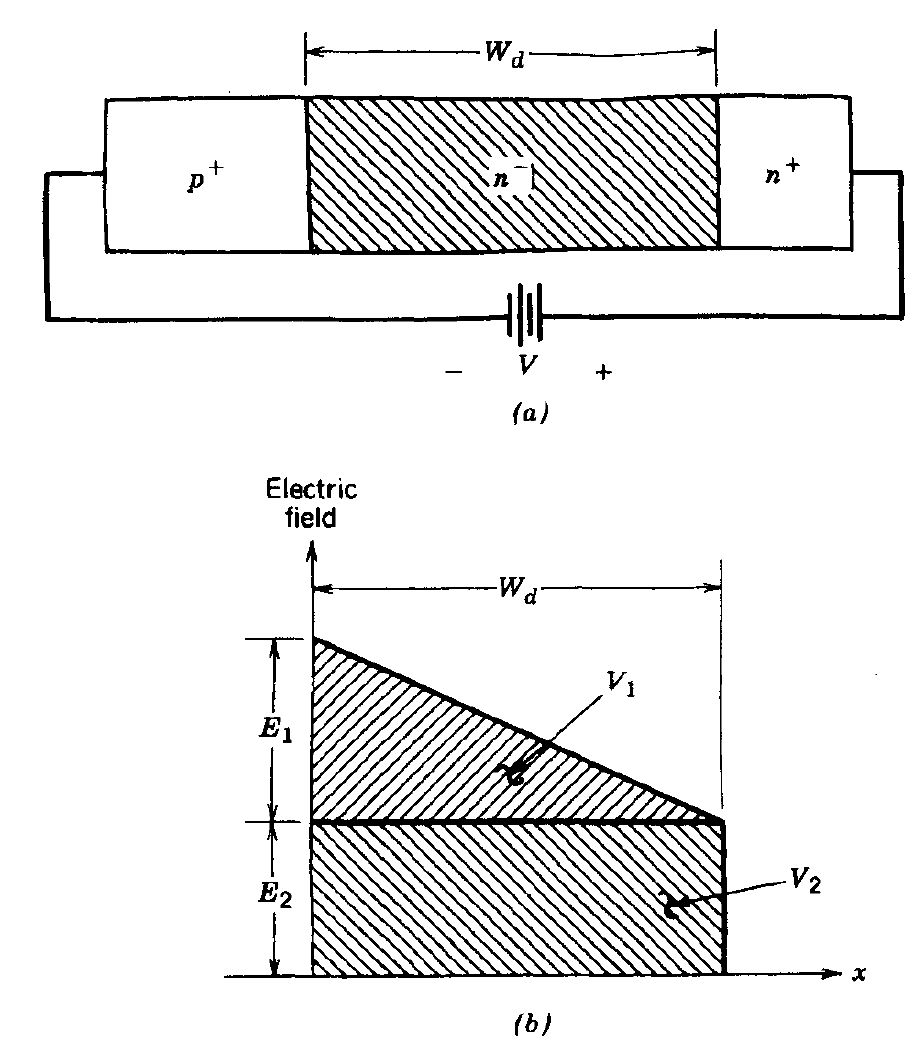
\includegraphics[scale=0.25]{fig/lec04/punch_through.png}
        \caption{\scriptsize Punch-through diode under reverse bias: (a) Depletion layer extends fully across the drift region (punch-through condition); (b) Electric field profile. Adapted from Mohan et al., \textit{Power Electronics, 2nd Ed.}}
        \label{fig:punch_through_diode}
    \end{figure}
    \end{column}
    
    \end{columns}
\end{frame}


\begin{frame}{\textbf{Electric Field \& Voltage Profile in Punch-Through Diode}}
    \begin{itemize}
        \item Electric field profile:
        \begin{itemize}
            \item Triangular portion: $E_1 = \frac{qN_dW_d}{\varepsilon}$
            \item Rectangular portion: $E_2$
        \end{itemize}
        \item Breakdown voltage:
        \begin{equation}
            V_1 = \frac{qN_dW_d^2}{2\varepsilon}, \quad V_2 = E_2 W_d
        \end{equation}
        \begin{equation}
            BV_{BD} = V_1 + V_2 = E_{BD}W_d - \frac{qN_dW_d^2}{2\varepsilon}
        \end{equation}
    \end{itemize}
    \textbf{Observation:} When $V_1 \ll V_2$, then $BV_{BD} \approx E_{BD}W_d$
\end{frame}

\begin{frame}{\textbf{Implications of Punch-Through Design}}
    \begin{itemize}
        \item Allows shorter $W_d$ for same $BV_{BD}$ → compact device.
        \item Higher resistivity in drift region increases $R_{on}$:
        \begin{itemize}
            \item Higher conduction loss compared to non-punch-through.
        \end{itemize}
        \item \textbf{Important:} No conductivity modulation under on-state — no conductivity injection from minority carriers.
        \item Results in higher $R_{on}$ under on-state condition.
    \end{itemize}
    \textbf{Conclusion:} Useful for high-speed, high-frequency operation despite higher on-resistance.
\end{frame}

\begin{frame}
    \frametitle{Power Diodes- Static characteristics}
    \begin{columns}
        \column{0.45\textwidth}
        \begin{itemize}
            \item \textbf{Linear forward conduction:}
            \begin{itemize}
                \item high forward current flows through the lightly doped drift region, introducing significant series resistance $R_{on}$.
                \item The characteristic is linear rather than exponential beyond $\approx$ 1V.
            \end{itemize}
            \item \textbf{Reverse bias and avalanche breakdown:}
            \begin{itemize}
                \item Under reverse bias, a small leakage current flows until the breakdown voltage $BV_{BD}$ is reached.
                \item Beyond $BV_{BD}$ avalanche multiplication causes current to rise rapidly while the voltage remains approximately constant.
            \end{itemize}
            \item \textbf{Breakdown operation must be avoided!.}
        \end{itemize}

        \column{0.55\textwidth}
        \begin{figure}
            \centering
            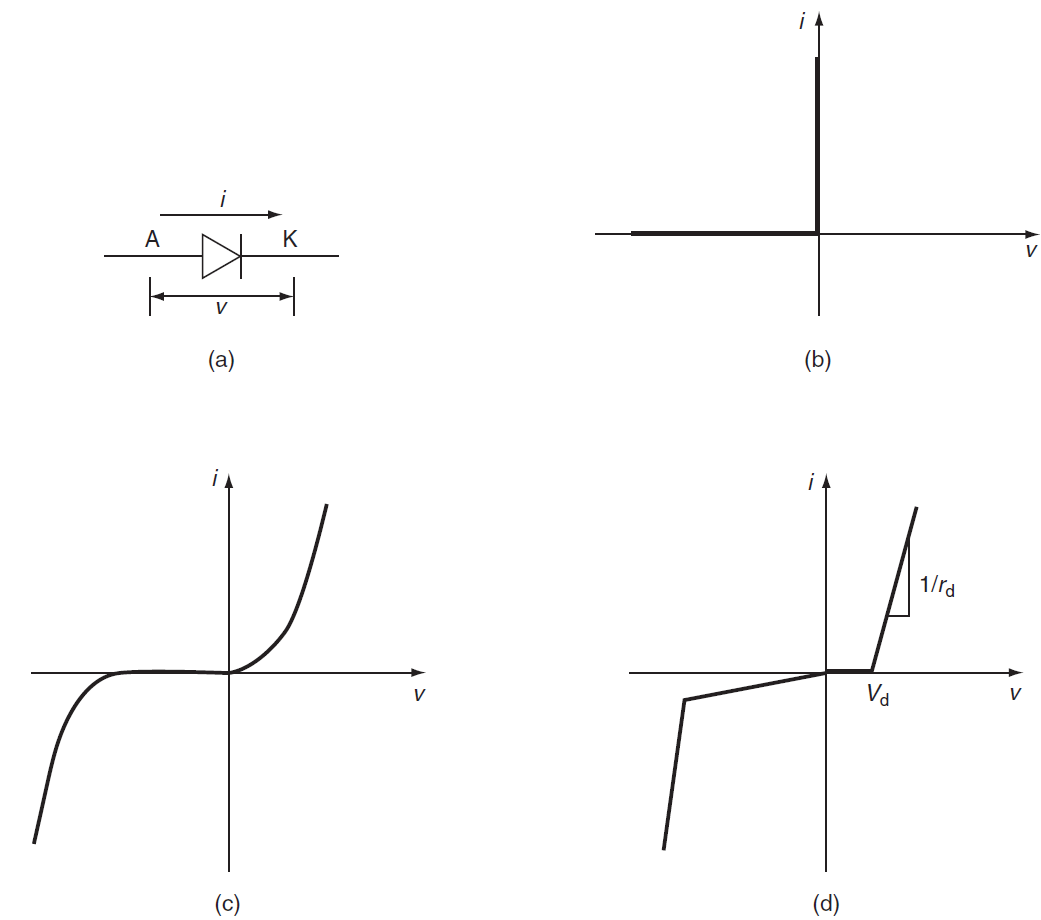
\includegraphics[scale=0.275]{fig/lec04/static_characteristics_diode.png}
            \caption{(a) symbol of diode, (b) ideal VI characteristics, (c) VI characteristics of a practical diode (d) piece wise linear model; adapted from Umanand, L., Power Electronics: Essentials \& Applications.}
            \label{fig:static_diode_characteristics}
        \end{figure}
    \end{columns}
\end{frame}

\begin{frame}
    \frametitle{Power Diodes- Dynamic characteristics}
    \begin{columns}
        \column{0.45\textwidth}
        \textbf{Turn-OFF of Diode:}
        \begin{itemize}
            \item When a forward-biased diode is suddenly reverse biased, excess carriers in the diffusion region (space-charge region) must be removed.
            \item The diode voltage remains in the ON-state initially due to stored charge.
            \item Reverse current flows until charges are removed at time $t_2$, after which the junction becomes reverse biased.
            \item The time interval from $t_1$ to $t_2$ is termed \textbf{storage time}, and $t_{rr}$ (total duration of reverse recovery) is crucial for switching applications.
        \end{itemize}
        \column{0.55\textwidth}
        \begin{figure}
            \centering
            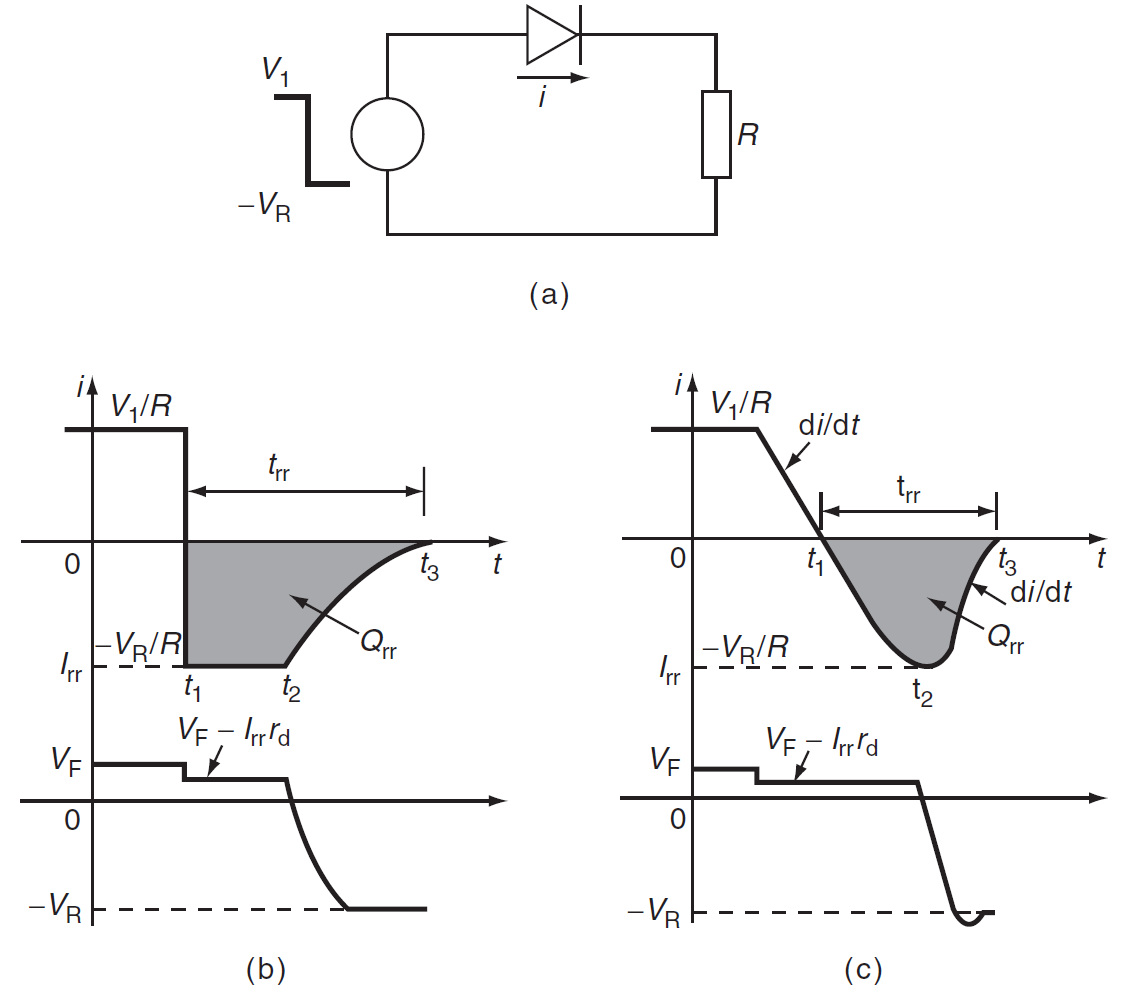
\includegraphics[scale=0.25]{fig/lec04/dynamic_characteristics_diode.png}
            \caption{(a) test circuit- turn-off, (b) ideal dynamic characteristics, (c) practical diode dynamic characteristics-turn-off; adapted from Umanand, L., Power Electronics: Essentials \& Applications.}
            \label{fig:dynamic_diode_characteristics}
        \end{figure}
    \end{columns}
\end{frame}

\begin{frame}
    \frametitle{Power Diodes- Dynamic characteristics}
    \begin{columns}
        \column{0.45\textwidth}
        \textbf{Turn-ON of Diode:}
        \begin{itemize}
            \item If a diode under reverse bias is forward biased, the transition requires a time known as \textbf{turn-ON time} or \textbf{forward recovery time}.
            \item Charges redistribute from to establish steady-state conduction.
            \item This process is generally faster than charge removal during turn-OFF, hence $t_{ON} < t_{OFF}$.
        \end{itemize}
        \vspace{0.2cm}
        \textit{Note: In practical circuits, reverse recovery can be slowed by parasitic inductance.}

        \column{0.55\textwidth}
        \begin{figure}
            \centering
            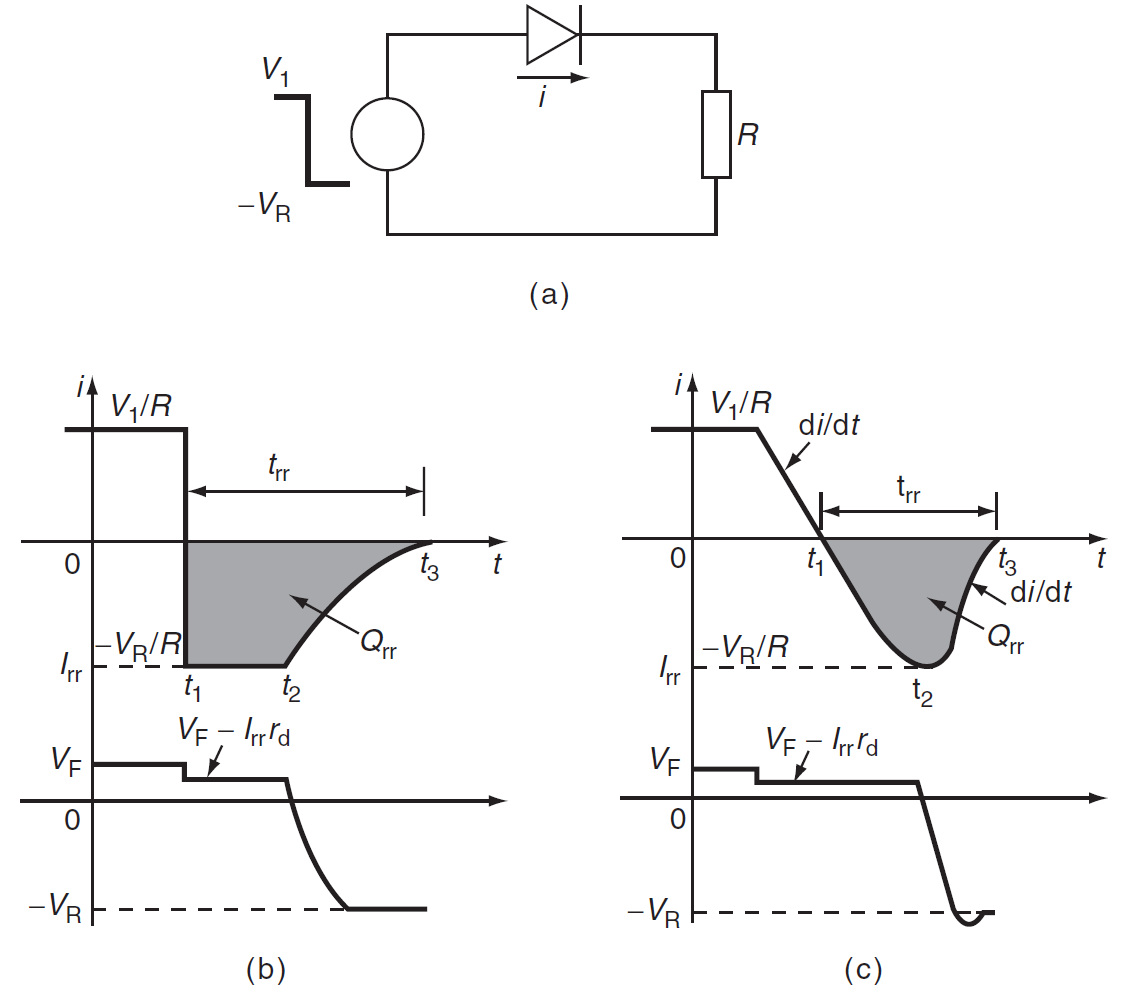
\includegraphics[scale=0.25]{fig/lec04/dynamic_characteristics_diode.png}
            \caption{(a) test circuit- turn-off, (b) ideal dynamic characteristics, (c) practical diode dynamic characteristics-turn-off; adapted from Umanand, L., Power Electronics: Essentials \& Applications.}
            \label{fig:dynamic_diode_characteristics}
        \end{figure}
    \end{columns}
\end{frame}

\begin{frame}{\textbf{Classification and Parameters of Power Diodes}}

    \textbf{Diode Classifications}
    \begin{itemize}
        \item Classification is based on reverse recovery time $t_{rr}$, indicating how quickly a diode can switch off.
        \item \textbf{Types of Diodes:}
        \begin{enumerate}
            \item \textbf{Rectifier Diodes:} $t_{rr}$ in the microsecond range.
            \item \textbf{Fast Recovery Diodes:} $t_{rr}$ between 200--500 ns.
            \item \textbf{Ultra-Fast Recovery Diodes:} $t_{rr} \sim$ 30--200 ns.
            \item \textbf{Schottky Diodes:} Metal-semiconductor junction, $t_{rr} <$ 30 ns.
        \end{enumerate}
        \item For high-frequency applications (e.g. SMPS, converters), use types 2--4 based on frequency and voltage ratings.
    \end{itemize}
    
    \textbf{Applications:}
    \begin{itemize}
        \item Type 1 is suitable for low-frequency mains rectification.
        \item Types 2--4 used in fast-switching converters.
    \end{itemize}
    
    \end{frame}
    
    \begin{frame}{\textbf{Datasheet Parameters for Diode Selection}}
    
    \textbf{Key Diode Parameters:}
    \begin{enumerate}
        \item Average forward current, $I_{\text{Fav}}$
        \item RMS forward current, $I_{\text{Frms}}$
        \item Peak forward current, $I_{\text{F}}$
        \item Surge current, $I_{\text{FSM}}$
        \item Breakdown or reverse voltage, $V_{\text{RRM}}$
        \item Forward voltage drop, $V_{\text{F}}$
        \item Dynamic resistance, $r_d$
        \item Reverse recovery time, $t_{rr}$
        \item Thermal endurance: $I^2t$ rating
    \end{enumerate}
    
    \textbf{Important Notes:}
    \begin{itemize}
        \item For sinusoidal operation, $I_{\text{Fav}}, I_{\text{Frms}}, I_{\text{F}}$ relations are well-known.
        \item For non-sinusoidal waveforms, these values must be derived from fundamentals.
        \item Choose diode ratings higher than the worst-case circuit values.
    \end{itemize}
    
    \end{frame}
    
    \begin{frame}{\textbf{Surge Current}}
        \textbf{Surge Current:}
        \begin{itemize}
            \item Diodes can handle overload currents briefly without damage.
            \item Key datasheet specs: $I_{\text{FSM}}$ (max peak half-cycle non-repetitive current) and $I^2t$ (energy dissipation).
            \item Surge current often arises when rectifier filters switch on with high peak voltages.
            \item Limiting devices (e.g., series resistors or fuses) ensure surge stays below $I^2t$ limit.
        \end{itemize}
    \end{frame}
        
\begin{frame}{\textbf{Thermal Viewpoint of Diodes}}
    \textbf{Thermal Viewpoint:}
    \begin{itemize}
        \item Total power loss: $P_d = P_{\text{on}} + P_{\text{off}} + P_{\text{switching}}$
        \item \textbf{On-state loss:}
        \begin{equation}
            P_{\text{on}} = \frac{1}{T} \int_0^T v(t)i(t)\, dt \approx (V_d \times I_{\text{avg}}) + (I_{\text{rms}}^2 \times r_d)
        \end{equation}
        \item \textbf{Switching loss:}
        \begin{equation}
            P_{\text{switching}} = E_{\text{switching}} \cdot f_s = \left( \frac{1}{2} Q_{\text{rr}} V_R \right) f_s
        \end{equation}
        \item Reverse recovery charge:
        \begin{equation}
            Q_{\text{rr}} = \frac{1}{2} t_{\text{rr}} I_{\text{rr}} \Rightarrow P_{\text{switching}} = \frac{1}{4} I_{\text{rr}} V_R t_{\text{rr}} f_s
        \end{equation}
        \item Junction temperature must remain below datasheet limit (e.g., 150$^\circ$C).
    \end{itemize}
\end{frame}


\begin{frame}{\textbf{Modeling a Power Diode: Steady-State and Transient Behavior}}
    \begin{columns}
        \begin{column}{0.48\textwidth}
            \textbf{Objective:} To model both static and dynamic characteristics of a diode for simulation and design purposes.
            \vspace{0.5em}
            \begin{itemize}
                \item \textbf{Steady-State Behavior:}
                \begin{itemize}
                    \item Current-voltage $(i_d$–$V_d)$ relationship is exponential:
                    \[
                        i_d = I_0\left(e^{\frac{V_d}{nV_T}} - 1\right)
                    \]
                    \item $R_s$: Series resistance due to bulk and contact resistance (non-zero in practice).
                \end{itemize}
            \end{itemize}
        \end{column}
        
        \begin{column}{0.48\textwidth}
            \begin{figure}
                \centering
                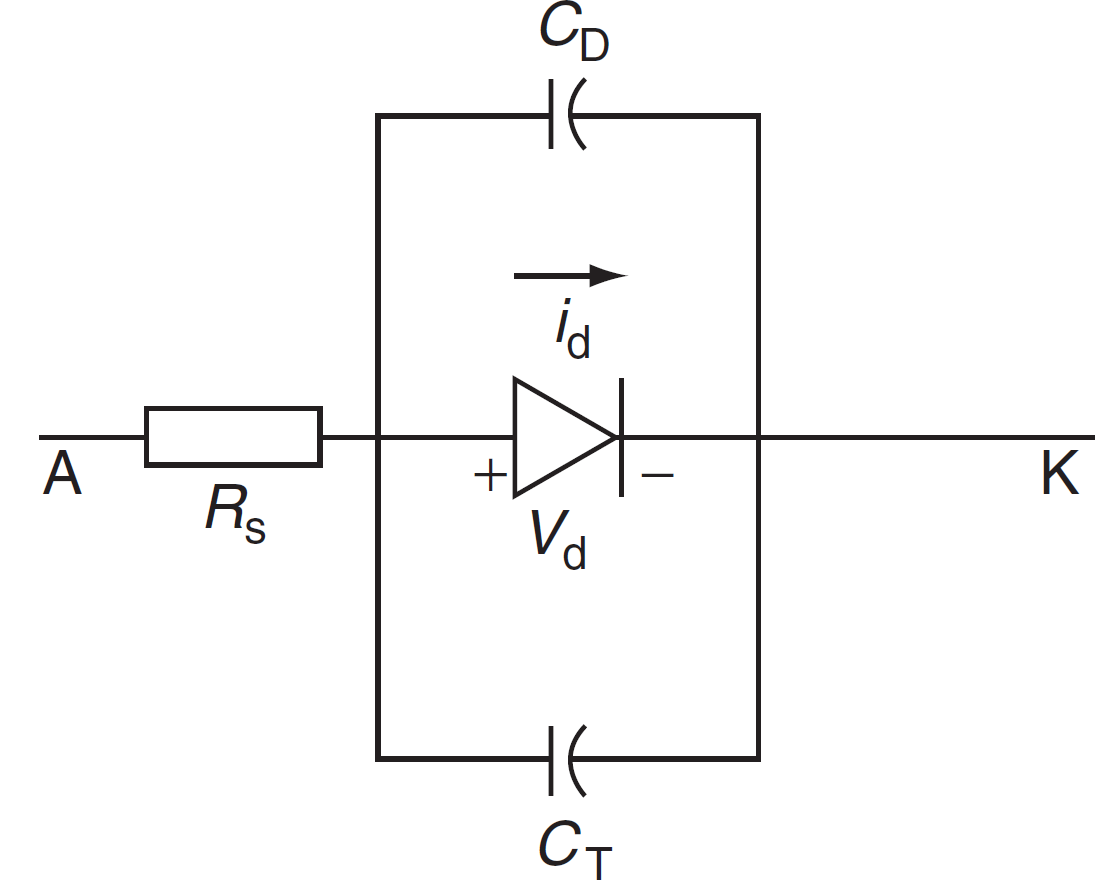
\includegraphics[scale=0.25]{fig/lec04/diode_model.png}
                \caption{Model of diode; adapted from Umanand, L., Power Electronics: Essentials \& Applications.}
                \label{fig:diode_model}
            \end{figure}
        \end{column}
    \end{columns}
    \end{frame}
    

\begin{frame}{\textbf{Modeling a Power Diode: Steady-State and Transient Behavior}}
    \begin{columns}
        \begin{column}{0.48\textwidth}
\begin{itemize}
\item \textbf{Dynamic Behavior:}
\begin{itemize}
    \item \textbf{Diffusion Capacitance ($C_D$):} 
        \begin{itemize}
            \item Appears during transition from forward to reverse bias.
            \item Models the excess mobile charge that must be removed.
        \end{itemize}
        
    \item \textbf{Transition Capacitance ($C_T$):}
        \begin{itemize}
            \item Relevant when transitioning from reverse to forward bias.
            \item Models mobile charge accumulation at the junction.
        \end{itemize}
\end{itemize}

\item \textbf{Capacitance Non-Linearity:}
    \begin{itemize}
        \item Both $C_D$ and $C_T$ are non-linear and depend on the charge distribution.
        \item Circuit simulators implement these models dynamically.
    \end{itemize}
\end{itemize}
\end{column}

\begin{column}{0.48\textwidth}
    \begin{figure}
        \centering
        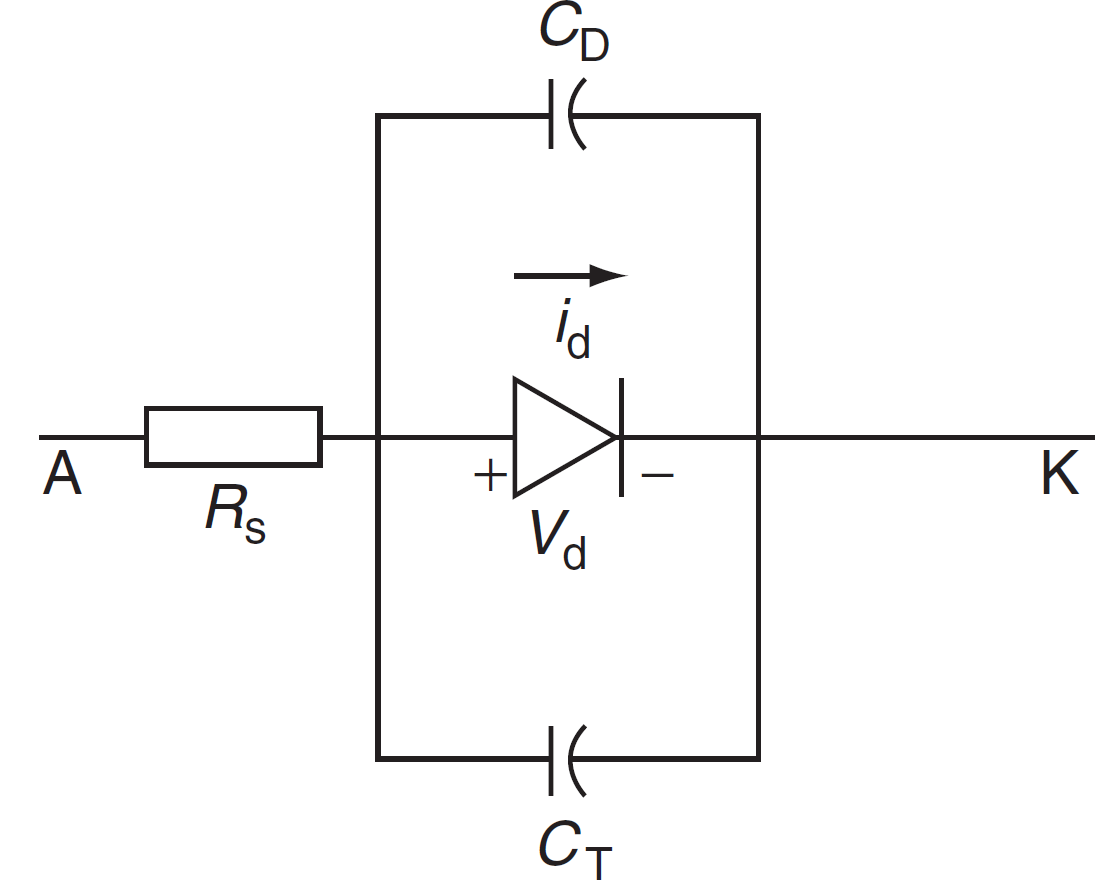
\includegraphics[scale=0.25]{fig/lec04/diode_model.png}
        \caption{Model of diode; adapted from Umanand, L., Power Electronics: Essentials \& Applications.}
        \label{fig:diode_model}
    \end{figure}
\end{column}
\end{columns}
\end{frame}